\chapter{Research Avenues \who{Axhausen, Nagel}}
\label{ch:researchavenues}
% ##################################################################################################################

\hfill \textbf{Authors:} Kai Nagel, Kay W.\ Axhausen

\begin{center} 
\includegraphics[width=0.3\textwidth, angle=0]{figures/MATSimBook.png} \end{center}

%%%%%%%%%%%%%%%%%%%%%%%%%%%%%%%%%%%%%%%%%%%%
%%%%%%%%%%%%%%%%%%%%%%%%%%%%%%%%%%%%%%%%%%%%
\section{\acrshort{matsim} and Agents}

% Q-learning: learn utility for each state-action pair
%
% utility learning: learn utility for each state
%
% difference: In the second case, need to have a model about the world.  I.e. need to know which actions lead to which probabilities for the next state.

% 20.2 passive learning in a known environment

% naive: proceed until terminal state, backpropagate utility to all previous states, average over all such utility values ever collected per state

% adaptive dynamic programming: U(i) = R(i) + \sum_j M_{ij} U(j)

% where R(i) is the reward at i and M_{ij} are the transition probas 
% (recall that this is passive learning)

% I don't that that this can be sampled ... needs to solve the equations

% temporal difference (TD) learning: U(i) <-- U(i) + alpha * ( R(i) + U(j) - U(i) ) 

% 20.3 passive learning in an unknown environment

% Since TD never neede M_{ij}, it will still work as before.  Will now also 
% learn M_{ij}, but separately

% 20.4 active learning in an unknown environment

% Now M^a_{ij} (depending on the action)

% U(i) = R(i) + max_a \sum_j M^a_{ij} U(j)

% TD approach same as before

% 20.5 Exploration

% 20.6 Learning an action-value function (Q values, Q-learning)

The core \acrshort{matsim} architecture -- where agents learn utilities for plans -- was originally derived from the so-called field of Complex Adaptive Systems (CAS).  
%
\cite{ArthurBar} addresses a coordination problem, where agents receive a payoff only when less than 60 out of 100 go to an event.  He addresses this by first generating a large number of heuristic predictors for the next round's attendance, such as ``same as in last round'' or ``trend of last four rounds''.  He next gives each agent a randomly selected handful of these strategies, so that agents in general have different sets of predictors.  Then, many rounds of the game are played, where the score of each predictor is updated based on its prediction quality, and agents act based on their currently best predictor.  Simulations demonstrate that the approach leads to successful coordination, i.e.\ around 60~agents show up in every round.
%
That approach in turn builds on work by \cite{PalmerEtAl_PhysicaD_1994}, who simulate a stock market,  \cite{Holland_1992}, whose classifier systems have more structure than Arthur's model but have a similar model of performance learning, or \cite{AxelrodBook}, who investigates adaptive agent in the face of repeated non-cooperative games.  

\citet{ArthurBar} kept each agent's predictors fixed after initialization.  In contrast,
\cite{HraberJonesForrestEcho} simulate an artificial ecosystem, where the individual agent strategies are based on so-called genes, which are adapted over the rounds/iterations by a genetic algorithms \citep{Goldberg_1989}.

The focus of CAS is on many agents, agent interaction, and emergence.  Artificial intelligence (AI) in contrast concentrated on single agents.  In AI terms, the original \acrshort{matsim} agents (those that do day-to-day learning) are very simple active reinforcement learning agents \citep[][Chapter 21.3]{RusselNorvig2010ArtificialIntelligence}.  Since these \acrshort{matsim} have only one state and each plan is simply an action, the distinction between Q-learning and utility learning actually collapses, and what remains is the temporal difference learning scheme for the utility, which translated to the \acrshort{matsim} situation updates the score/performance/utility value of each plan every time it is selected.

That is, overall, the original \acrshort{matsim} system has inherited the focus on large systems, interaction, and emergence as well as the approach to strategy innovation from CAS, while the score updating rather comes from the field of AI.

In the meantime, both AI and the field of transport simulation have moved on, increasingly looking at agents that can react immediately, rather than having to wait for the next iteration or round.  In transport, this is sometimes called en-route or within-day replanning \citep[e.g.][]{EmmerinkEtAl_TransResC_1995,balijepalli-2007}.

\kai{to do more}



%%%%%%%%%%%%%%%%%%%%%%%%%%%%%%%%%%%%%%%%%%%%
%%%%%%%%%%%%%%%%%%%%%%%%%%%%%%%%%%%%%%%%%%%%
\section{Within-Day Replanning and the User Equilibrium}
\label{sec:researchavenues-withinday}

\vfill\eject
%%%%%%%%%%%%%%%%%%%%%%%%%%%%%%%%%%%%%%%%%%%%
%%%%%%%%%%%%%%%%%%%%%%%%%%%%%%%%%%%%%%%%%%%%
\section{Frozen randomness}

a horni

\vfill\eject
%%%%%%%%%%%%%%%%%%%%%%%%%%%%%%%%%%%%%%%%%%%%
%%%%%%%%%%%%%%%%%%%%%%%%%%%%%%%%%%%%%%%%%%%%
\section{Choice set generation}
\label{sec:choicesets}

\kai{in particular plans removal!! From Benjamin's diss:}

In the plans innovation process of the simulation, the plan with the lowest utility is removed whenever the maximum number of plans are reached for an agent. In consequence, this decreases the probability that heterogeneous plans survive and increases the probability of very similar plans. This, again, increases the likelihood that the final choice set is correlated, i.e.\ containing only plans that are very similar to the best plan \citep[see][for a review on correlation of 
 routes]{Prato2009ChoiceModellingSurvey}.%
 %
 \footnote{
 %
 A possible solution to this problem is most likely composed of two steps:
 %
 First, more heterogeneity needs to be introduced into the choice set generation, e.g.\ by producing very different plans.
 %
 Second, the method for plans removal needs to be based on an \gls{mnl} model where the difference in utility enters, similar to the approach of selecting plans for execution. This could be done by an implementation of a method called `pathsize logit' which uses similarity measures for plans \citep[see][for a possible solution in route choice]{FrejingerBierlaire2007PathSizeLogit, BenAkivaBierlaiere1999DiscreteChoice}.
 %
 }

---

To give recommendations to other researchers: the bias in choice set generation of \gls{matsim} needs to be fixed in the near future in order to obtain valid choice sets.
%
This requires (i) the generation of more heterogeneous plans \citep[see, e.g.,][for such attempts in the \acrshort{pt} and in the car mode, respectively]{Moyo2013PhD, NagelKickhoeferJoubert2014HeterogeneousVoTsPROCEDIA}; and (ii) the implementation of a pathsize logit model in the plans removal process \citep[see, e.g.,][]{Grether2014PhD}.
%
Having obtained these valid choice sets \citep{NagelFloetteroed2009IatbrResourceInBook}, the calculation of user benefits based on the logsum formulation is preferable.
%
\benjamin{Well, here it now depends on how we write the previous section...}
%
Using the logsum formulation with correlated choice sets requires a careful interpretation of the results. However, when looking at differences between the two states before and after a policy, this issue is unlikely to change results structurally: if the correlation remains roughly the same between the two states, the error of utility differences is small. If the correlation structure of plans changes, the error will\textemdash among other model specifications\textemdash depend on the number of iterations.
%
\benjamin{If we iterate the base case to the same iteration number as the policy case, the former will be more correlated. This would result in a underestimation of the utility changes.}
%
In that sense, one could include some approximation of the error into the analysis of results, possibly similar to Eq.~\ref{eq:ch:economicEval:logsumMaxError}. If the differences in utility levels between the two states are in the same magnitude as $\ln(P)$, it is possible that the signal of the policy effect is smaller than the noise of randomness.

%%%%%%%%%%%%%%%%%%%%%%%%%%%%%%%%%%%%%%%%%%%%
%%%%%%%%%%%%%%%%%%%%%%%%%%%%%%%%%%%%%%%%%%%%
\section{Utility function}
\label{sec:future-of-scoring-function}

\kai{In particular: calibration of 2nd derivative!}

\subsection{Estimating a Utility Function}
\label{sec:estimation}
\ah{With the exception of \citet[][]{BalmerEtAl_ResRep_datapuls_2010}, the estimates by \citet[][]{Kickhoefer_MastersThesis_2009} have not been considered for the various calibrations and extensions mentioned above although it represents a valuable base for further estimations. Having such a base at hand is important as estimating and applying a MATSim utility function is non-trivial due to the following. 

The agents optimize complete day plans \citep[see also][Section 6.3.1]{MATSim_Userguide_2014}. This means that the single choice dimension utility terms need to neatly fit into the complete function. It is not possible to apply functions estimated independently for only a single choice dimensions. If for example all alternatives for destination choice evaluated with an inappropriate utility function generate negative utility, then the complete activity is simply dropped. This correlation or dependency between choice dimensions is also the reason why a day plan equilibrium does not necessarily include a Nash equilibrium for every single choice dimensions. The inseparability of choice dimensions means that in MATSim we can only consistently handle choices if we assume an absolute utility level rather than a relative level usually assumed for discrete choice models. 

Incorporating an extension, for example for parking or destination choice, in combination with absolute utilities becomes even more tricky as the Charypar-Nagel function is non-linear, which means that available models very often being linear, need to be incorporated by workarounds such as approximation procedures and distinction of cases as described in \citet[][p.75ff]{Horni_PhDThesis_2013}. Furthermore, it is based on travel times, which is usually seen as an unreliable information gathered from classical surveys. GPS or smartphone-based surveys, however, provide this information with great precision and, thus, they are advantageously used for future estimations.

Furthermore, travel time and activity duration estimations including income need to carefully consider the parameters' relation to the value of travel time savings. \citet[][p.276]{MeisterEtAl_SVT_2009} for example argues that the average Swiss hourly earnings are much higher than $6\ EUR/h$. However, the MATSim is measured in utils not monetary units anymore. But still, the parameters in utils and monetary terms (such as tolls, parking costs, fares etc., or income-dependent attributes) are often interacted and thus their relation needs to be consistent.

A numerical problem, particularly relevant for activity choice, concerns the functional form of the utility function. As argued in \citet[][p.33]{MATSim_Userguide_2014}, a function offering an additional degree of freedom (the curvature at the typical duration) would be better.

Estimating a utility function for MATSim is associated with another problem. The function is applied iteratively for a travel demand which is in the beginning of the relaxation process usually not very similar to the situation where the function was estimated. In other words, the function is used for a whole range of working points, where it has been estimated for only one  possibly completely different working point. The MATSim function thus must be also correct in the elasticities, to be able to efficiently drive the relaxation process toward the final relaxation point, where the estimated function is valid by construction. 
}

\subsection{Agent-Specific Preferences:}
\label{sec:agent-specific-prefs}
\ah{In project Surprice \citet[][]{HorniEtAl_TechRep_IVT_2012_a, HorniAxhausen_TechRep_IVT_2014}, agent-specific travel preferences and individual income-dependent marginal utilities of money are incorporated. It is simulated with a 1\% multi-modal Zürich scenario, the preference values however, are assigned randomly. }

\subsection{S-Shaped Function and Its Estimates:}
\label{sec:s-shaped-function}
\ah{Both \citet[][p.127f]{Feil_PhDThesis_2010} and \citet[][p.32]{MATSim_Userguide_2014} report that the standard logarithmic function of MATSim is not suitable for modeling activity sequence choice. Due to the log form very short activities are favored, which means that the schedule is filled-up with numerous short activities, where the usually long home activities are replaced first. Since this is unrealistic behavior, a new function was introduced by \citet[][p.129ff]{Feil_PhDThesis_2010}. The function is based on \citet[][]{Joh_PhDThesis_2004} and is asymmetrically S-shaped. First estimates of the new function based on the Swiss microcensus were provided, which were calibrated for the schedule recycling functionality by \citet[][p.152f]{Feil_PhDThesis_2010}. The function was not developed further.}


\vfill\eject
%%%%%%%%%%%%%%%%%%%%%%%%%%%%%%%%%%%%%%%%%%%%
%%%%%%%%%%%%%%%%%%%%%%%%%%%%%%%%%%%%%%%%%%%%
\section{Results Variability}
\label{sec:variability}
Microsimulation system design as well as concrete microsimulation studies require specification of the measures \kai{quantities?} of interest.\footnote{%
Formal system specification (and verification) is discussed e.g., in \citet[][]{FisherWooldridge_IJCIS_1997, BourahlaBenmohamed_ENTCS_2005}. 
} For microsimulation design, they need to be general and broadly available, count data are an example. For specific experiments and purposes other measures might be added; \citet[][]{Kitamura_TMIP_1996}, for example, lists measures relevant for emissions modeling. Considering their scale is important for model development, but a certain lack of research exists in this regard. \citet[][Section 2.2]{NagelAxhausen_TechRep_IVT_2001}, for example, say: ``Another question regarding scales is which scale is necessary to answer which question. There is wide-spread intuition but currently little hard knowledge. Rules-of-thumb, such as to include one level of resolution below the level of interest, are just rule-of-thumb.'' 

Scale of the measures of interest is also relevant for results production, as different scales or resolution levels usually lead to different levels of \emph{variability} and, thus, to different study costs in terms of required computation effort. Transport microsimulations are usually stochastic. Randomness is, for example, introduced by the error terms of discrete choice models, a common component in utility-based microsimulations. This leads to random variability in results. Parameters or population statistics, such as averages, thus, need to be estimated by random sampling. Microsimulations are thus essentially a sampling tool \citep[][]{WolfDA_CSP_2001}, where one run represents one sample unit (in statistical terms one \emph{realization of a random variable}). This makes clear, that the whole toolbox used for other statistical methods, must be applied also here. As a first step, required sample size---here, the number of runs---to ensure a given confidence in the calculated averages needs to be calculated. In this context, variability is often seen as something tedious, because higher variability leads to larger minimal sample sizes, with usually relatively high costs per sample point. But, this view falls short. Clearly, unobserved variability---modeled as random variability---should be replaced to the extent possible (by explaining it). However, when looking at the very large proportion of temporal variability actually present in reality (Figure \ref{fig:counts}), a substantial part of this variability is---even if it was actually explicable---much more efficiently handled by including randomness, as model complexity would be prohibitively large otherwise. In this sense, microsimulations are a tool to capture these real-world fluctuations \citep[][p.11]{NewmanMEJBarkema_1999}, \citep[][p.704]{EsserNagel_Hensher_2001}. This means also that the focus should not only be on averages, but also on variance incorporated in the calculations of statistical confidence. The following sections broaden the microsimulation variability analysis.

\createfigure[T]%
{Measured volumes}%
{Volumes. LEFT: Reality.  RIGHT: Simulation. \kai{Hallo Andreas, mitteln die Messungen aus der Realität über alle Tagestypen einschl.\ Samstag, Sonntag, Ostern, Weihnachten, etc.?} \kai{Falls ja, so würde ich sagen, dass das dann ohnehin schwer zu vergleichen ist, und auch erklärt, was man sieht: In den realen Daten vor allem die Schwankungen zwischen den Tagestypen, womit dann die ``daily'' Schwankungen nicht kleiner sind als die ``hourly''.  In der Simulation hingegen Monte Carlo noise, der erwarteterweise kleiner wird, wenn man über 24h mittelt.}}%
{\label{fig:counts}}%
{%
% ===
	\createsubfigure%
  {Daily Volumes}%

{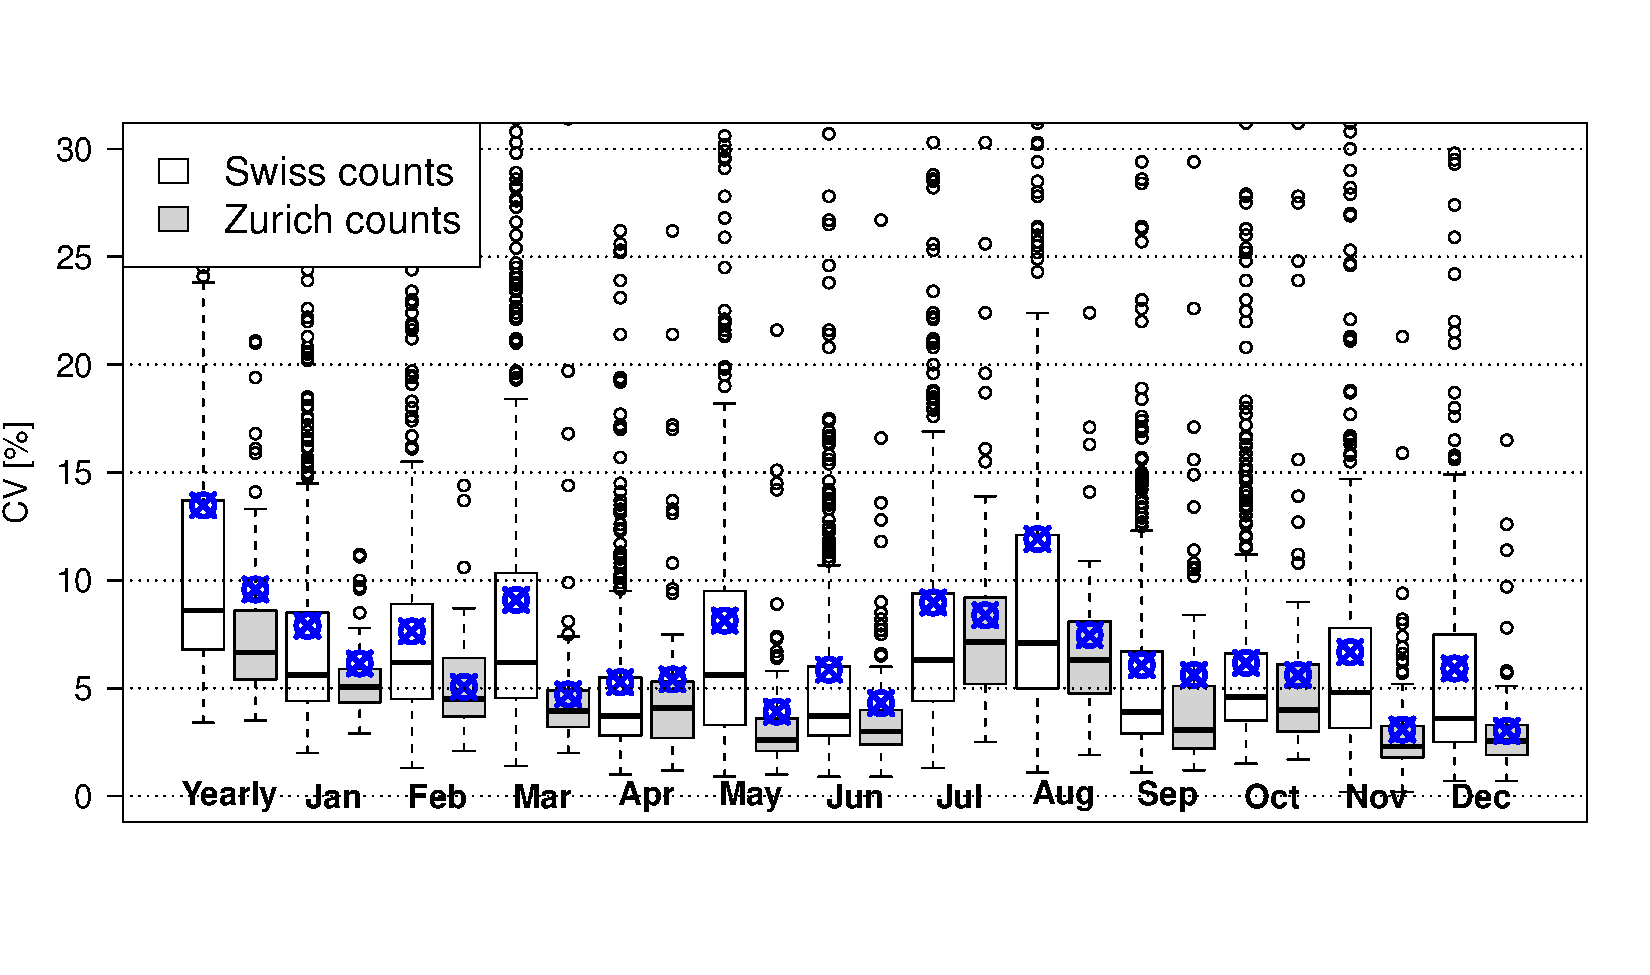
\includegraphics[height=0.3\textwidth]{understanding/figures/var/countsDaily.pdf}}%
	{\label{fig:countsDaily}}%
  {}%
% ---
	\createsubfigure%
  {Simulated Daily Volumes: Inter-run Variability, Runs 0-29, Iteration 200}%
	{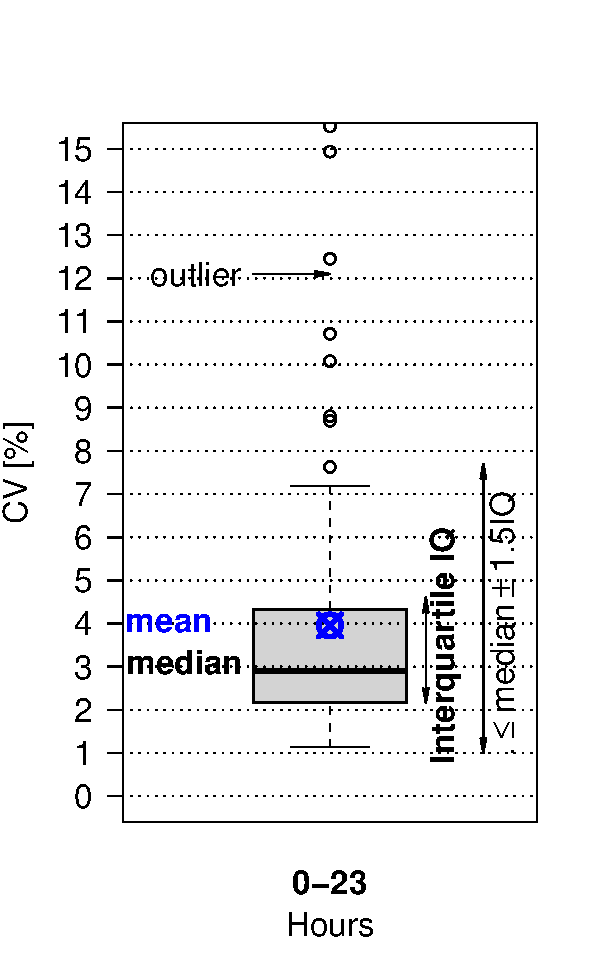
\includegraphics[height=0.3\textwidth]{understanding/figures/var/linkVolumesInterAWTV200.pdf}}%
	{\label{fig:linkVolumesInterAWTV200}}%
  {}%
% ===
  \createsubfigure%
  {11:00-12:00}%
	{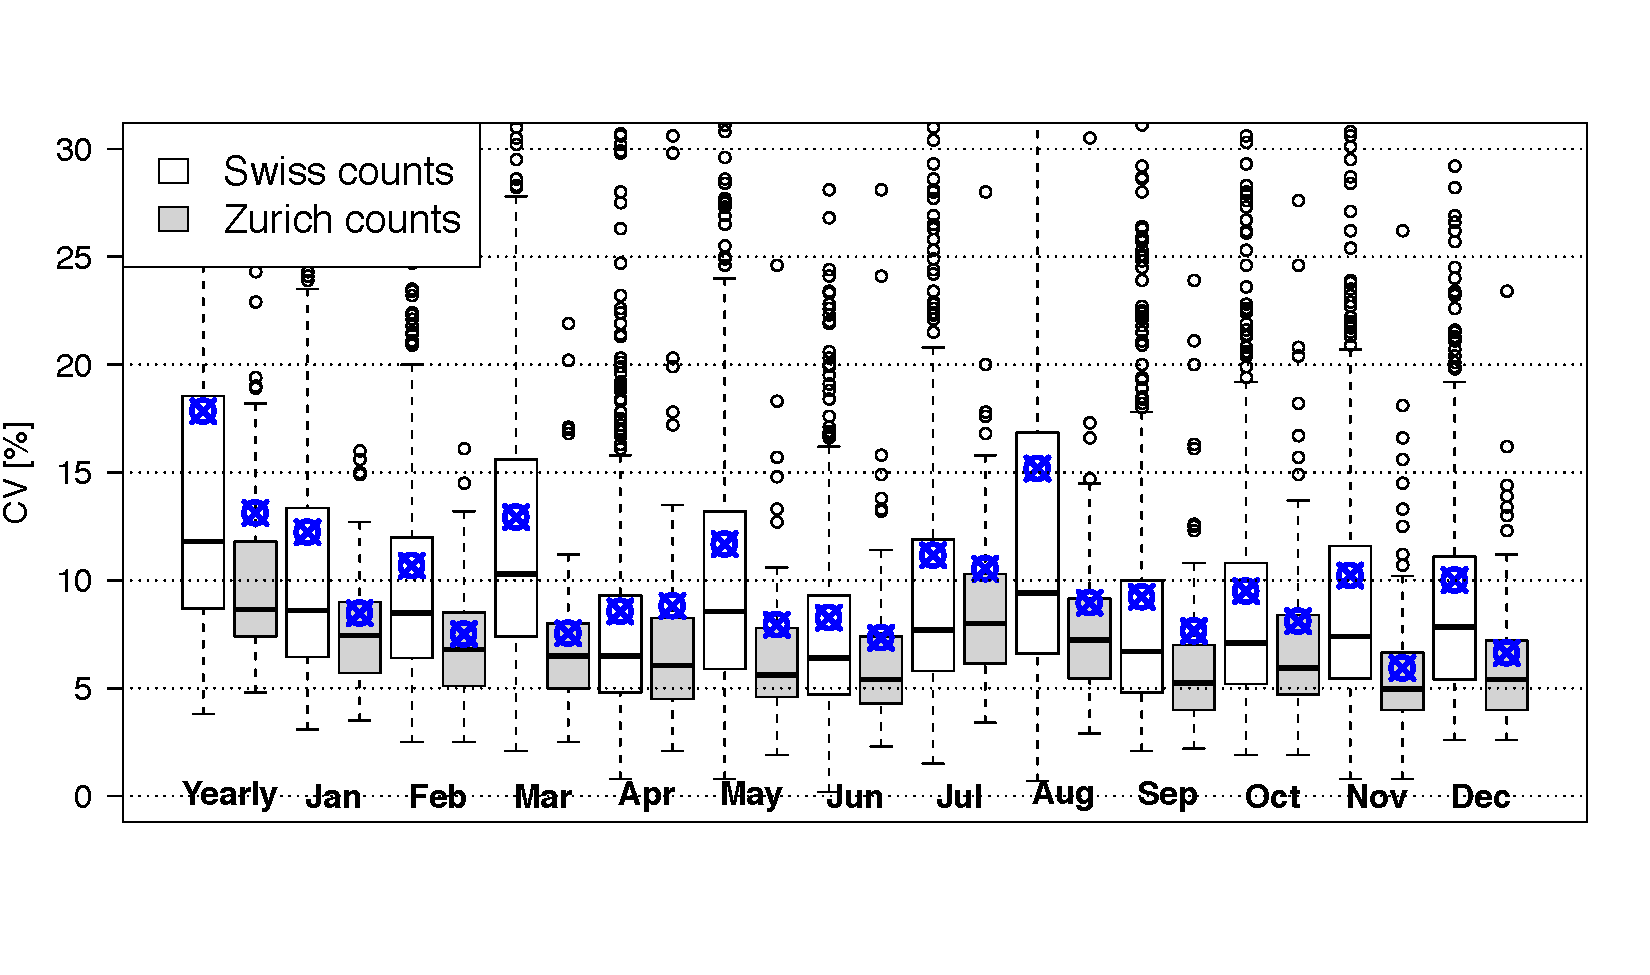
\includegraphics[height=0.3\textwidth]{understanding/figures/var/counts11-12.pdf}}%
	{\label{fig:H1112}}%
  {}%
% ---
	\createsubfigure%
  {Simulated Hourly Volumes: Inter-run Variability, Runs 0-29, Iteration 200}%
	{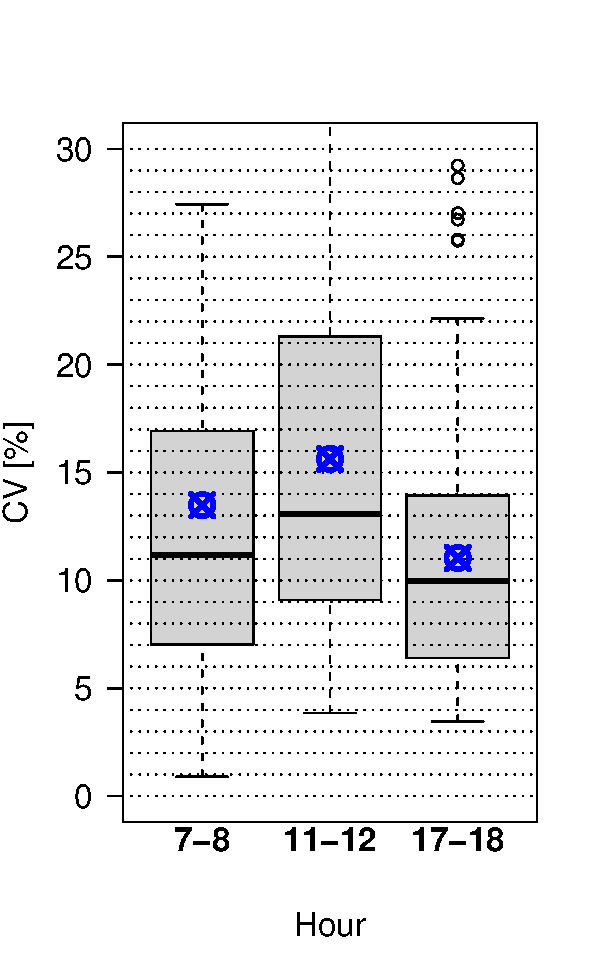
\includegraphics[height=0.3\textwidth]{understanding/figures/var/linkVolumesInter200.pdf}}%
	{\label{fig:linkVolumesInter200}}%
  {}%
% ===
 	\createsubfigure%
  {17:00-18:00}%
	{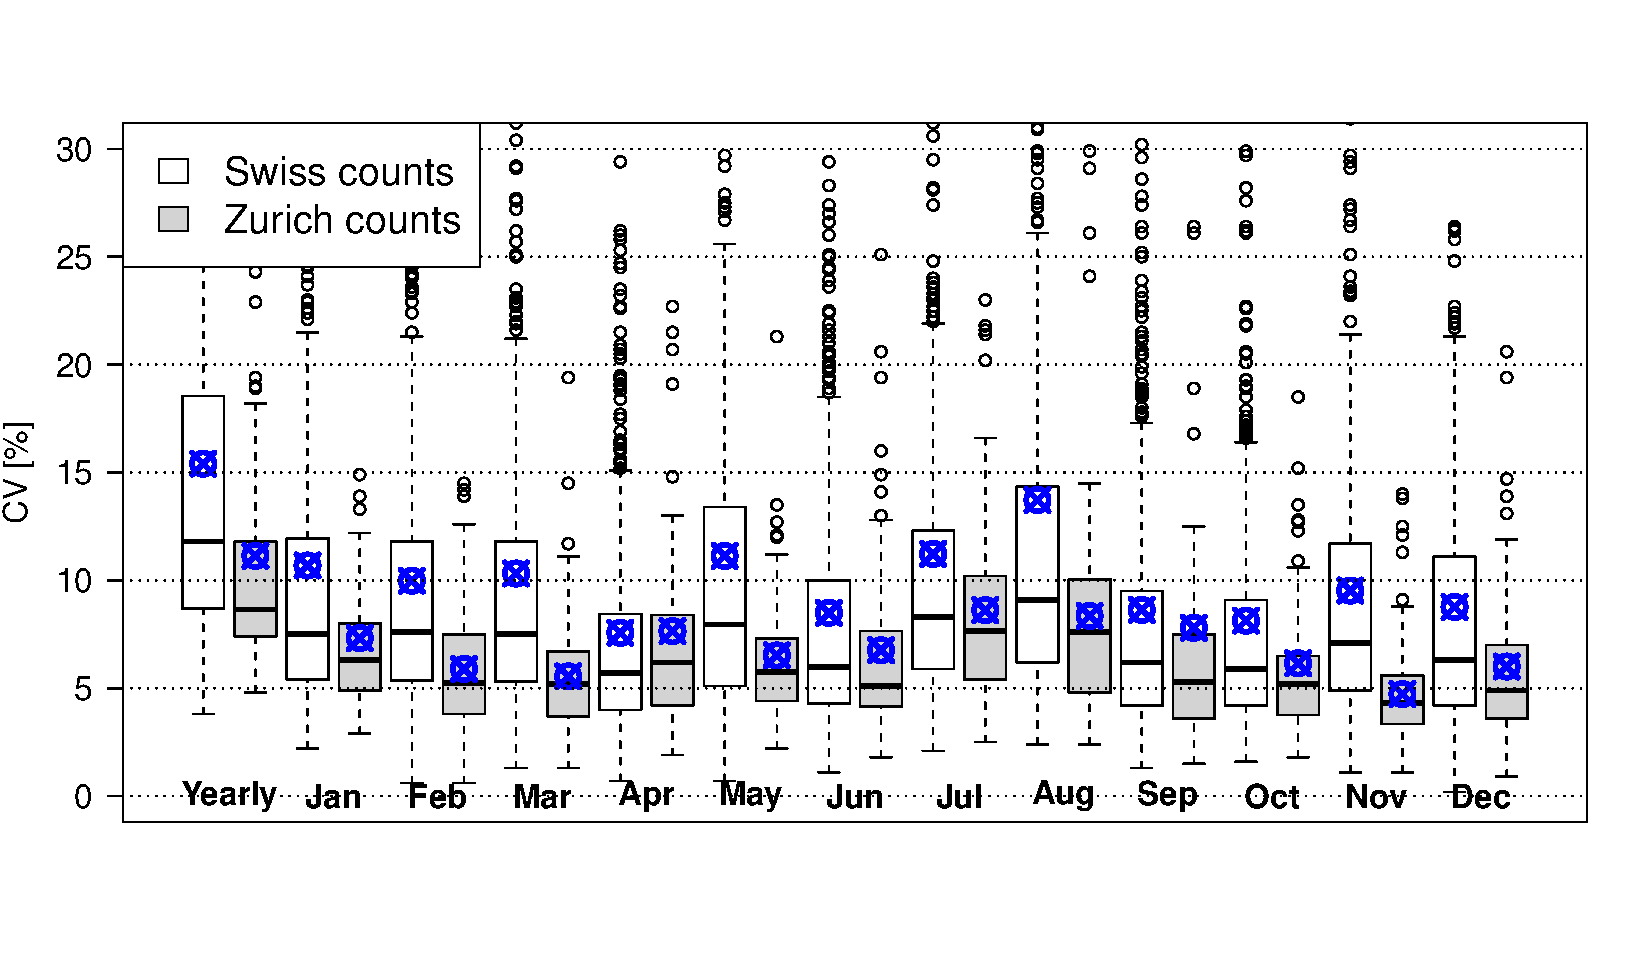
\includegraphics[height=0.3\textwidth]{understanding/figures/var/counts17-18.pdf}}%
	{\label{fig:H1718}}%
  {}%
% ---
	\createsubfigure%
  {Simulated Hourly Volumes: Inter-run Variability, Runs 0-29, Iteration 200}%
	{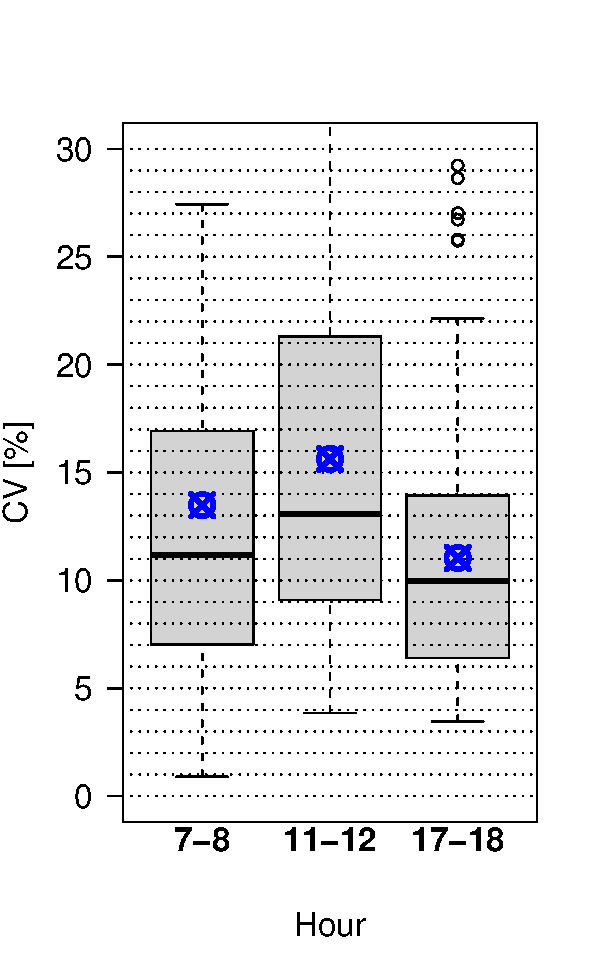
\includegraphics[height=0.3\textwidth]{understanding/figures/var/linkVolumesInter200.pdf}}%
	{\label{fig:linkVolumesInter200}}%
  {}%
% ===
}%
{}

Multiple possibilities to categorize microsimulations variability exist; some categories are described by \citet[][]{HorniEtAl_TechRep_IVT_2011_b}. Often a distinction between endogenous (model) variability and exogenous (input) variability is made. Equally suitable one can distinguish systematic and random variability. The experiments reported below mainly focus on \emph{random, endogenous} model variability. Random variability stems from inherently random choices and from actually systematic choices not recognized as systematic by the modeler.

MATSim variability was investigated by \citet[][]{HorniEtAl_TechRep_IVT_2011_b, HorniEtAl_STRC_2011, Dayte_TechRep_IVT_2012} coming to the conclusion that at the population level, as expected, there is little variability between simulation results. Little variability exists likewise for \emph{daily} volumes as shown in Figures \ref{fig:linkVolumesAWTVInterScatter} and \ref{fig:linkVolumesInterAWTV200} (with a different visualization), which is consistent with previous work. However, the variability for \emph{hourly} volumes is an issue as shown in Figures~\ref{fig:linkVolumesHour17-18InterScatter} and Figure~\ref{fig:linkVolumesInter200} (with a different visualization).

To interact these substantial simualtion variability with variability observed in reality, \citet[][]{HorniEtAl_STRC_2011} looked at real-world link volumes given for both, the complete year and single months, meaning that a single point in the box plot represents temporal variability of a single network link, either for the whole year, or for a specific month. The hours 11-12 and 17-18 are shown as examples in Figure~\ref{fig:counts}, where similar patterns could be observed for all hours. The plots allow the conclusion that also in reality variability is also substantial.

Further MATSim investigations are reported by \citet[][]{Hackney_PhDThesis_2009, Neumann_PhDThesis_2014}.

\createfigure%
{Simulated link volumes}%
{Simulated link volumes}%
{\label{fig:linkVolumes}}%
{%
  \createsubfigure%
  {Simulated Daily Volumes: Inter-run Variability}%
	{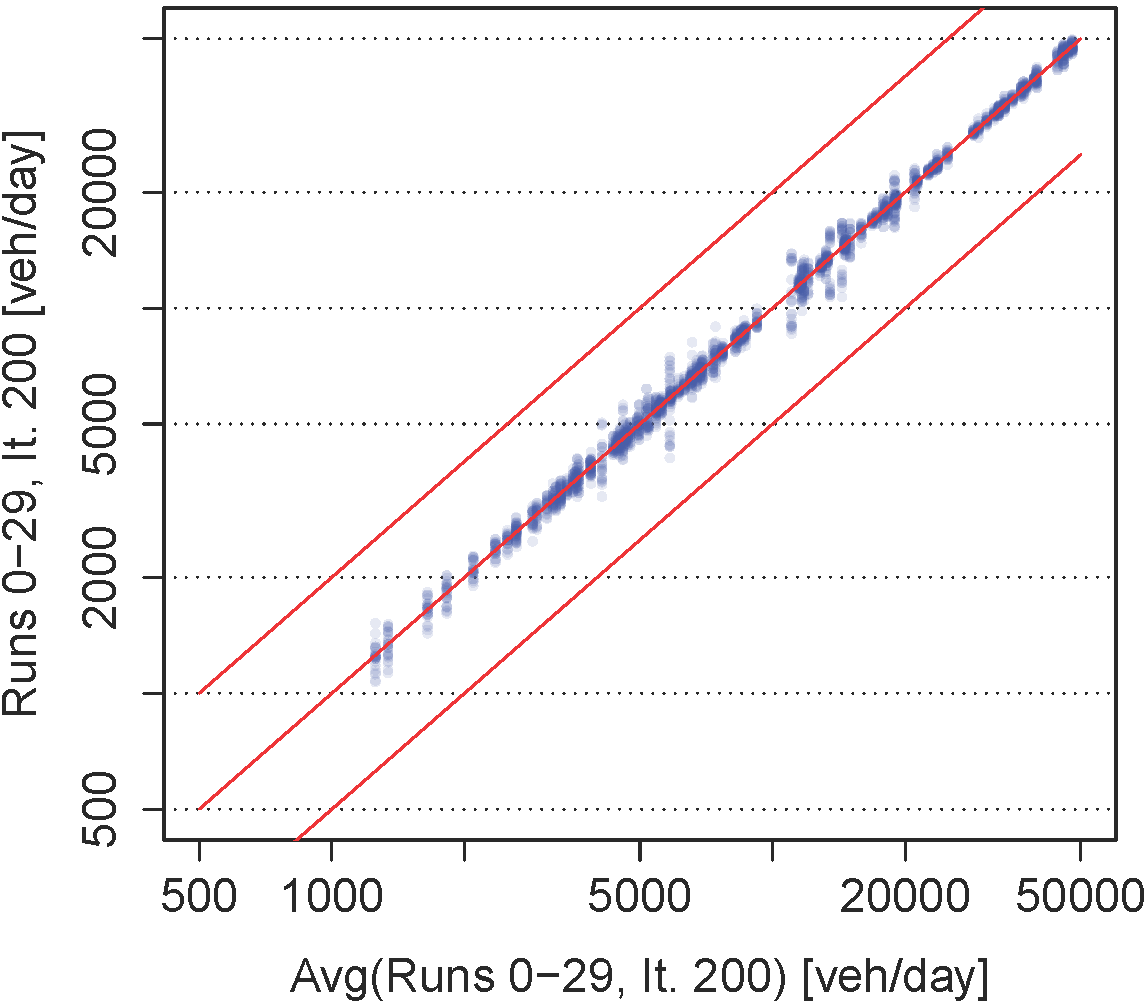
\includegraphics[width=0.49\textwidth]{understanding/figures/var/linkVolumesAWTVInterScatter.png}}%
	{\label{fig:linkVolumesAWTVInterScatter}}%
  {}%
	\createsubfigure%
  {Simulated Daily Volumes: Inter-run Variability, Runs 0-29, Iteration 200}%
	{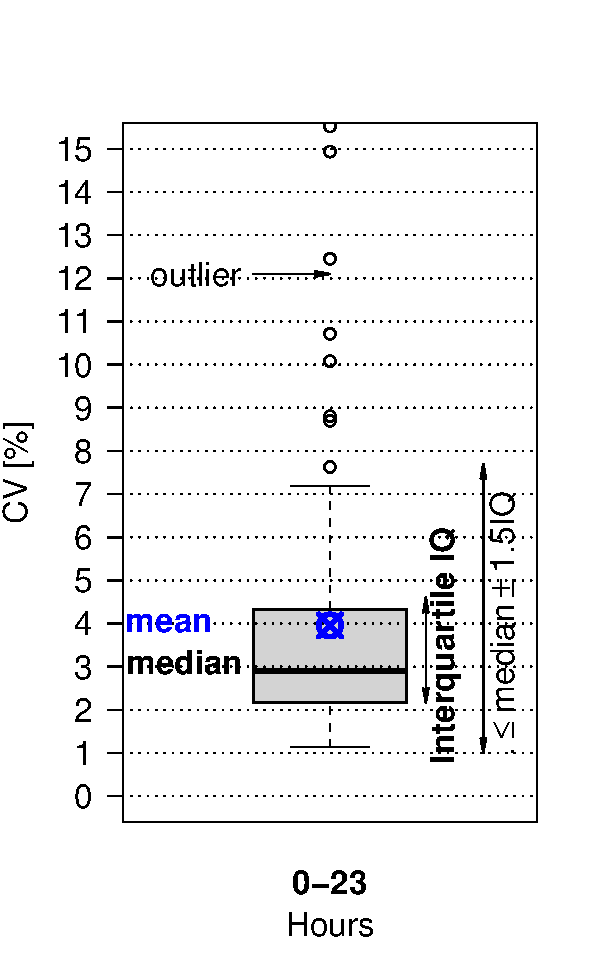
\includegraphics[width=0.3\textwidth]{understanding/figures/var/linkVolumesInterAWTV200.pdf}}%
	{\label{fig:linkVolumesInterAWTV200}}%
  {}%
  \createsubfigure%
  {Simulated Hourly Volumes (Hour 17-18), Inter-run Variability}%
	{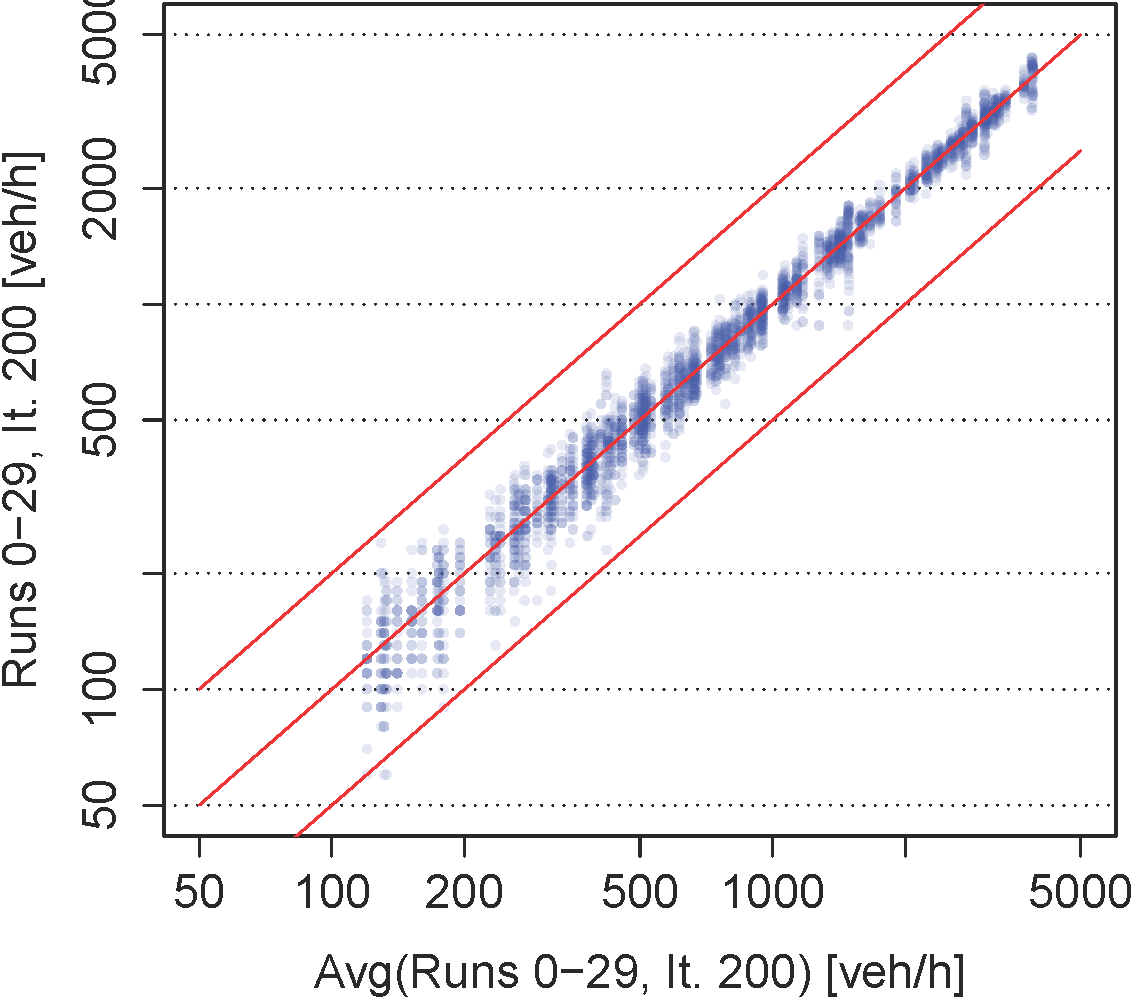
\includegraphics[width=0.49\textwidth]{understanding/figures/var/linkVolumesHour17-18InterScatter.png}}%
	{\label{fig:linkVolumesHour17-18InterScatter}}%
  {}%
	\createsubfigure%
  {Simulated Hourly Volumes: Inter-run Variability, Runs 0-29, Iteration 200}%
	{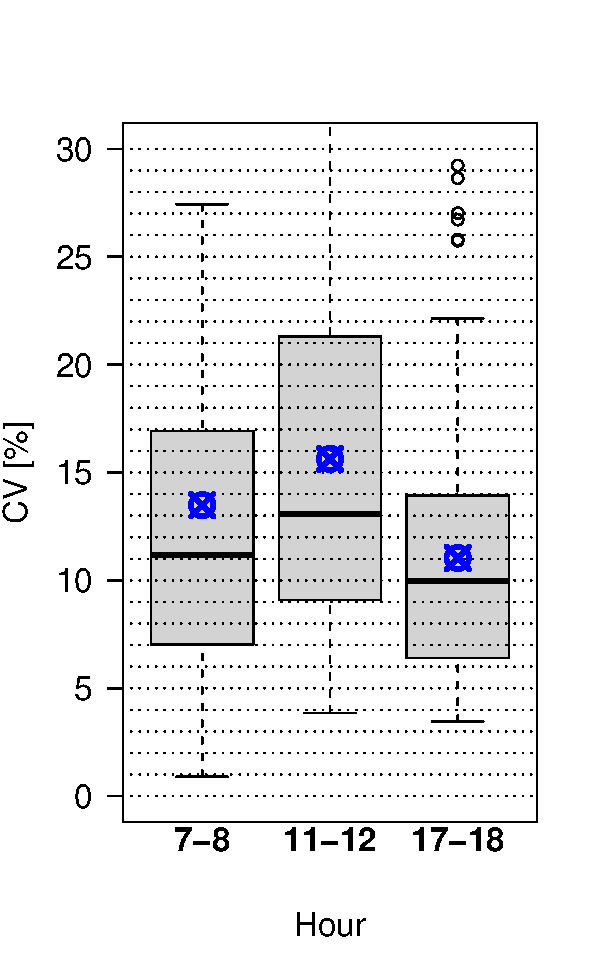
\includegraphics[width=0.3\textwidth]{understanding/figures/var/linkVolumesInter200.pdf}}%
	{\label{fig:linkVolumesInter200}}%
  {}%
}%
{} 

\vfill\eject
%%%%%%%%%%%%%%%%%%%%%%%%%%%%%%%%%%%%%%%%%%%%
%%%%%%%%%%%%%%%%%%%%%%%%%%%%%%%%%%%%%%%%%%%%
\section{Transients vs.\ the notion of ``learning''}
\label{sec:transients-vs-learning}

As in many other simulations of similar kind, the interpretation of the relaxation procedure (iterations) of MATSim is unclear. 
%
Sometimes the relaxation process is ascribed a behavioral interpretation, for example, day-to-day learning, where also the transition process and not only the final equilibrium has a meaning \citep[][p.128]{LiuEtAl_TransResA_2006}, \citep[][p.523]{NagelBarrett_IJMPC_1997}. 
%
An opposite perspective exists, where the relaxation procedure is just a numerical method to compute the equilibrium state or states without behavioral basis of the transitions.


\vfill\eject
%%%%%%%%%%%%%%%%%%%%%%%%%%%%%%%%%%%%%%%%%%%%
%%%%%%%%%%%%%%%%%%%%%%%%%%%%%%%%%%%%%%%%%%%%
% Local Variables:
% mode: latex
% mode: reftex
% mode: visual-line
% TeX-master: "main"
% comment-padding: 1
% fill-column: 9999
% End: 
